% -----------------------------------------------------------------------------
%DIF LATEXDIFF DIFFERENCE FILE
%DIF DEL main_v3.tex   Fri May 29 15:58:30 2026
%DIF ADD main_v4.tex   Fri May 29 15:55:49 2026
%DIF 2c2
%DIF < % main_v3.tex — third draft of the Tethys data paper.
%DIF -------
% main_v4.tex — fourth draft of the Tethys data paper. %DIF > 
%DIF -------
%
%DIF 4-9c4-22
%DIF < % v3 incorporates the v2 review pass: abstract reframed to lead with sector-
%DIF < % level biases, validation metrics table added, citation keys cleaned to
%DIF < % author-year style, Methods reorganized per coauthor request to lead with
%DIF < % scenarios + exogenous forcings before Tethys mechanics. Companion documents:
%DIF < %   - EQUATIONS_AUDIT.md  — per-equation reconciliation of paper vs code
%DIF < %   - STYLE_NOTES.md      — distilled voice/structure from 3 Bracken SciData papers
%DIF -------
% v4 incorporates the v3 review round (REVIEW.md, the v3-2026-05-29 independent %DIF > 
% review, and Wenwei's COAUTHOR_COMMENTS.md). Highlights vs v3: %DIF > 
%   - Validation Table 2 numbers replaced with values from the actual pipeline %DIF > 
%     (compute-table2-metrics.py); n=329 HUC6 basins; bias signs reconciled. %DIF > 
%   - Skinner2025USGS bib key renamed to Harris2025 (first author is Harris). %DIF > 
%   - Eq. 5 HDD/CDD threshold sensitivity test added. %DIF > 
%   - Figure 1 flow chart redrawn natively in TikZ; per Wenwei's comment a %DIF > 
%     "Tethys" box now wraps Spatial + Temporal Downscaling, Demeter scale %DIF > 
%     annotated, "Monthly Climate Variables" -> "Monthly Meteorological %DIF > 
%     Variables", PET/HDD/CDD/GSI spelled out in caption. %DIF > 
%   - Dominant water-use sector map promoted to flagship figure (now Figure 1) %DIF > 
%     with a Background & Summary in-text reference. %DIF > 
%   - val6 scenarios timeseries regenerated so the historical line connects to %DIF > 
%     the future scenario lines (no visual gap at 2020). %DIF > 
%   - Backup PNGs preserved for figures that were updated. %DIF > 
% Companion documents: %DIF > 
%   - EQUATIONS_AUDIT.md  -- per-equation reconciliation of paper vs code %DIF > 
%   - STYLE_NOTES.md      -- distilled voice/structure from 3 Bracken SciData papers %DIF > 
%   - RESPONSE_TO_COMMENTS_v3.md -- review-by-review reconciliation %DIF > 
%DIF -------
%
% Open issues flagged for coauthor resolution:
%   - Author list ordering and affiliation numbering (please verify).
%DIF 13-15c26-28
%DIF < %   - Author CRediT statement (lines 438+) is illustrative; needs coauthor pass.
%DIF < %   - Validation table values for Domestic/Electricity/Irrigation should be
%DIF < %     re-verified against the validation pipeline before submission.
%DIF -------
%   - Author CRediT statement is illustrative; needs coauthor pass. %DIF > 
%   - Eq. 8 clip three numbers (basin-level mass-balance residual) -- Bracken %DIF > 
%     to verify; flagged in RESPONSE_TO_COMMENTS_v3.md. %DIF > 
%DIF -------
% -----------------------------------------------------------------------------

\documentclass[fleqn,10pt]{wlscirep}
\usepackage[utf8]{inputenc}
\usepackage[T1]{fontenc}
\usepackage{lineno}
\usepackage{booktabs}
%DIF 23a36-37
\usepackage{tikz} %DIF > 
\usetikzlibrary{positioning, arrows.meta, fit, backgrounds, shapes.geometric} %DIF > 
%DIF -------

\linenumbers

% \title{High-resolution 21st-century monthly water demands for the contiguous United States}
\title{High-resolution monthly sectoral water demands for the U.S., 1980-2100} % across diverse futures

\author[1*]{Cameron Bracken}
\author[2*]{Hassan Niazi}
\author[1]{Travis Thurber}
\author[2]{Isaac Thompson}
\author[1]{Kazi Tamaddun}
\author[3]{Hisham Eldardiry}
\author[1]{Kendall Mongird}
\author[1,3]{Nathalie Voisin}
\author[1]{Ning Sun}
\author[1]{Jennie Rice}

\affil[1]{Pacific Northwest National Laboratory, Richland, WA, USA}
\affil[2]{Joint Global Change Research Institute, Pacific Northwest National Laboratory, College Park, MD, USA}
\affil[3]{University of Washington, Seattle, WA, USA}

\affil[*]{corresponding author(s): Cameron Bracken (cameron.bracken@pnnl.gov), Hassan Niazi (hassan.niazi@pnnl.gov)}

\begin{abstract}
%DIF 47c62
%DIF < U.S. water demand varies sharply by sector and region as climate, land use, population, and economic activity co-evolve. We present a gridded (1/8$^{\circ}$), monthly, multi-sector water demand dataset for the contiguous United States (CONUS) covering 1980--2100 across one historical period and eight future scenarios. Aggregate CONUS annual demand agrees with USGS 2015 estimates within 10\%, but this agreement is misleading: the dataset underestimates domestic demand by up to 45\% and thermoelectric withdrawals by up to 30\%, biases that are offset by a +5\% bias in irrigation. This dataset advances prior global products by combining GCAM-USA state-resolved sectoral demands, CERF-based future power-plant siting, and scenario-consistent high-resolution climate and population forcing. The fine-scale spatiotemporal patterns it provides support integrated energy-water-land modeling and local-to-regional water scarcity assessments across the eight scenarios.
%DIF -------
U.S. water demand varies sharply by sector and region as climate, land use, population, and economic activity co-evolve. We present a gridded (1/8$^{\circ}$), monthly, multi-sector water demand dataset for the contiguous United States (CONUS) covering 1980--2100 across one historical period and eight future scenarios. The dataset reproduces the spatial pattern of USGS 2010--2020 water-use observations with HUC6 Pearson correlations of 0.73--0.95 across Domestic, Electricity, and Irrigation withdrawals; aggregate per-sector mean bias errors are within $\pm 7\%$, but normalized RMSE and median absolute percent error remain large (68--171\% NRMSE, 37--86\% MedAPE) because per-basin biases compensate at the CONUS aggregate. This dataset advances prior global products by combining GCAM-USA state-resolved sectoral demands, CERF-based future power-plant siting, and scenario-consistent high-resolution climate and population forcing. The fine-scale spatiotemporal patterns it provides support integrated energy-water-land modeling and local-to-regional water scarcity assessments across the eight scenarios. %DIF > 
%DIF -------
\end{abstract}
%DIF PREAMBLE EXTENSION ADDED BY LATEXDIFF
%DIF UNDERLINE PREAMBLE %DIF PREAMBLE
\RequirePackage[normalem]{ulem} %DIF PREAMBLE
\RequirePackage{color}\definecolor{RED}{rgb}{1,0,0}\definecolor{BLUE}{rgb}{0,0,1} %DIF PREAMBLE
\providecommand{\DIFadd}[1]{{\protect\color{blue}\uwave{#1}}} %DIF PREAMBLE
\providecommand{\DIFdel}[1]{{\protect\color{red}\sout{#1}}} %DIF PREAMBLE
%DIF SAFE PREAMBLE %DIF PREAMBLE
\providecommand{\DIFaddbegin}{} %DIF PREAMBLE
\providecommand{\DIFaddend}{} %DIF PREAMBLE
\providecommand{\DIFdelbegin}{} %DIF PREAMBLE
\providecommand{\DIFdelend}{} %DIF PREAMBLE
\providecommand{\DIFmodbegin}{} %DIF PREAMBLE
\providecommand{\DIFmodend}{} %DIF PREAMBLE
%DIF FLOATSAFE PREAMBLE %DIF PREAMBLE
\providecommand{\DIFaddFL}[1]{\DIFadd{#1}} %DIF PREAMBLE
\providecommand{\DIFdelFL}[1]{\DIFdel{#1}} %DIF PREAMBLE
\providecommand{\DIFaddbeginFL}{} %DIF PREAMBLE
\providecommand{\DIFaddendFL}{} %DIF PREAMBLE
\providecommand{\DIFdelbeginFL}{} %DIF PREAMBLE
\providecommand{\DIFdelendFL}{} %DIF PREAMBLE
%DIF COLORLISTINGS PREAMBLE %DIF PREAMBLE
\RequirePackage{listings} %DIF PREAMBLE
\RequirePackage{color} %DIF PREAMBLE
\lstdefinelanguage{DIFcode}{ %DIF PREAMBLE
%DIF DIFCODE_UNDERLINE %DIF PREAMBLE
  moredelim=[il][\color{red}\sout]{\%DIF\ <\ }, %DIF PREAMBLE
  moredelim=[il][\color{blue}\uwave]{\%DIF\ >\ } %DIF PREAMBLE
} %DIF PREAMBLE
\lstdefinestyle{DIFverbatimstyle}{ %DIF PREAMBLE
	language=DIFcode, %DIF PREAMBLE
	basicstyle=\ttfamily, %DIF PREAMBLE
	columns=fullflexible, %DIF PREAMBLE
	keepspaces=true %DIF PREAMBLE
} %DIF PREAMBLE
\lstnewenvironment{DIFverbatim}[1][]{\lstset{style=DIFverbatimstyle}}{} %DIF PREAMBLE
\lstnewenvironment{DIFverbatim*}[1][]{\lstset{style=DIFverbatimstyle,showspaces=true}}{} %DIF PREAMBLE
\lstset{extendedchars=\true,inputencoding=utf8}

%DIF END PREAMBLE EXTENSION ADDED BY LATEXDIFF

\begin{document}

\flushbottom
\maketitle
% Click the title above to edit the author information and abstract

\thispagestyle{empty}

% -----------------------------------------------------------------------------
\DIFaddbegin \begin{figure}[ht]
\centering

\includegraphics[width=\linewidth]{usage1-dominant-sector-tethys-grid.png}
\caption{\DIFaddFL{Dominant water-use sector at each 1/8$^{\circ}$ cell across CONUS, by annual-average consumption in the historical Tethys output (1980--2019). The dataset resolves a complex multi-sector mosaic --- irrigation across the Great Plains, Mountain West, and Central Valley; thermoelectric concentrated near major generation centers in the Southeast and along the major navigable rivers; public-supply demand peaking around metropolitan areas; livestock, manufacturing, and mining adding regional structure --- that prior global products could not capture at this resolution. Each pixel is the sector with the largest annual-average consumption at that cell.}}
\label{fig:dominant-sector}
\end{figure}

\DIFaddend \section*{Background \& Summary}

Humans depend on water for irrigation, thermoelectric cooling, public supply, industry, and livestock. The relative importance of these sectors varies sharply across regions and over time. Global water demand has continued to rise through the 21st century under combined socioeconomic and climatic pressures\cite{WWDR2019, Niazi2024PeakWater, Awais2024Preprint}, and demand-side drivers, not supply-side limits, dominate most projected shifts in water scarcity\cite{Graham_2020, Awais2024Preprint, Kyle2023Sustainability}. Even where regional supply appears ample, scarcity can manifest locally when demand and availability are mismatched in space or time\cite{HADJIMICHAEL23}. Modeling scarcity under climate and socioeconomic change therefore requires demand resolved at the spatial and temporal scales of management decisions.

High-resolution, multi-sector water-demand projections remain scarce, constraining integrated modeling. Reconstructed historical datasets, such as Huang et al. (2018)\cite{Huang2018}, provide gridded benchmarks for past decades but do not extend to future scenarios. Global water scarcity assessments use coarse-resolution integrated assessment model outputs that lack the spatial detail required for river routing or local management modeling\cite{Wada_2017, van_Vliet_2021}. Bridging these scales requires spatial and temporal downscaling\cite{hess-17-4555-2013, van_Vliet_2021, Jones_2024}, but the choice of gridded proxy variables and the consistency of driving scenarios materially affect the resulting demand fields. Khan et al. (2023)\cite{Khan2023} produced the first global Tethys-downscaled multi-sector product at 1/2$^{\circ}$ monthly resolution; resolving CONUS-scale management decisions, however, requires finer spatial resolution and scenario-consistent climate, land-use, and population forcing.

We present such a dataset here, refined to 1/8$^{\circ}$ resolution across CONUS. The published record contains gridded monthly water withdrawals and consumption for six sectors: irrigation, thermoelectric, municipal (public-supply and domestic), livestock, manufacturing, and mining. The spatial resolution is 1/8$^{\circ}$, on the CONUS extent $[25.0625^{\circ}\text{N},\,52.9375^{\circ}\text{N}] \times [-124.9375^{\circ}\text{W},\,-67.0625^{\circ}\text{W}]$, for one historical period (1980--2019) and eight future scenarios (2020--2100) that vary by RCP, Thermodynamic Global Warming (TGW) climate sample, and Shared Socioeconomic Pathway (SSP). For each scenario the dataset also provides per-cell renewable vs.\ non-renewable source shares. The downscaling chain improves on the prior Tethys CONUS product in six specific ways (see Section~``Improvements over previous version''): GCAM-USA integration, explicit CERF-based\cite{Vernon2021} power-plant siting, SSP-consistent population proxies, climate-forced irrigation temporal downscaling using TGW-WRF derived deficits and growing-season indices (GSI), USGS-anchored source-share adjustment, and resolution refinement from 1/2$^{\circ}$ to 1/8$^{\circ}$. The dataset supports MultiSector Dynamics (MSD) research on U.S.\ bulk-power-system resilience, groundwater sustainability, and regional climate extremes by providing a shared scenario-consistent demand foundation that enables inter-model comparisons across MSD analyses. Figure~\DIFaddbegin \DIFadd{\ref{fig:dominant-sector} shows the dominant sector at each 1/8$^{\circ}$ cell across CONUS in the historical record --- the multi-sector mosaic this dataset captures and that motivates the rest of the paper. Figure~}\DIFaddend \ref{fig:schematic} shows the \DIFdelbegin \DIFdel{overall workflow }\DIFdelend \DIFaddbegin \DIFadd{workflow that produces it}\DIFaddend . Table~\ref{tab:prior-datasets} compares this dataset with closely related published records.

\begin{figure}[ht]
\centering
%DIF <  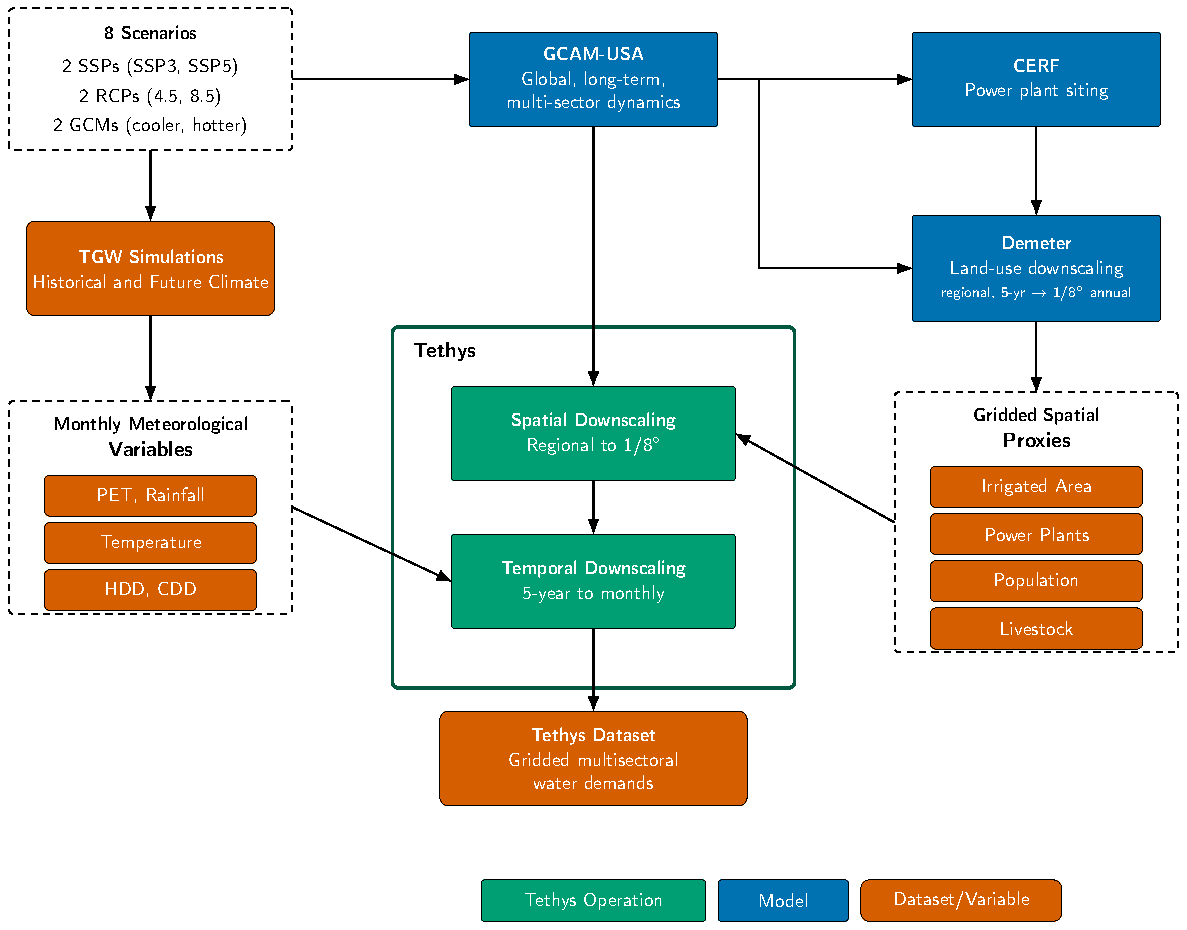
\includegraphics[width=0.85\linewidth]{flow-chart}
\DIFdelbeginFL %DIFDELCMD < 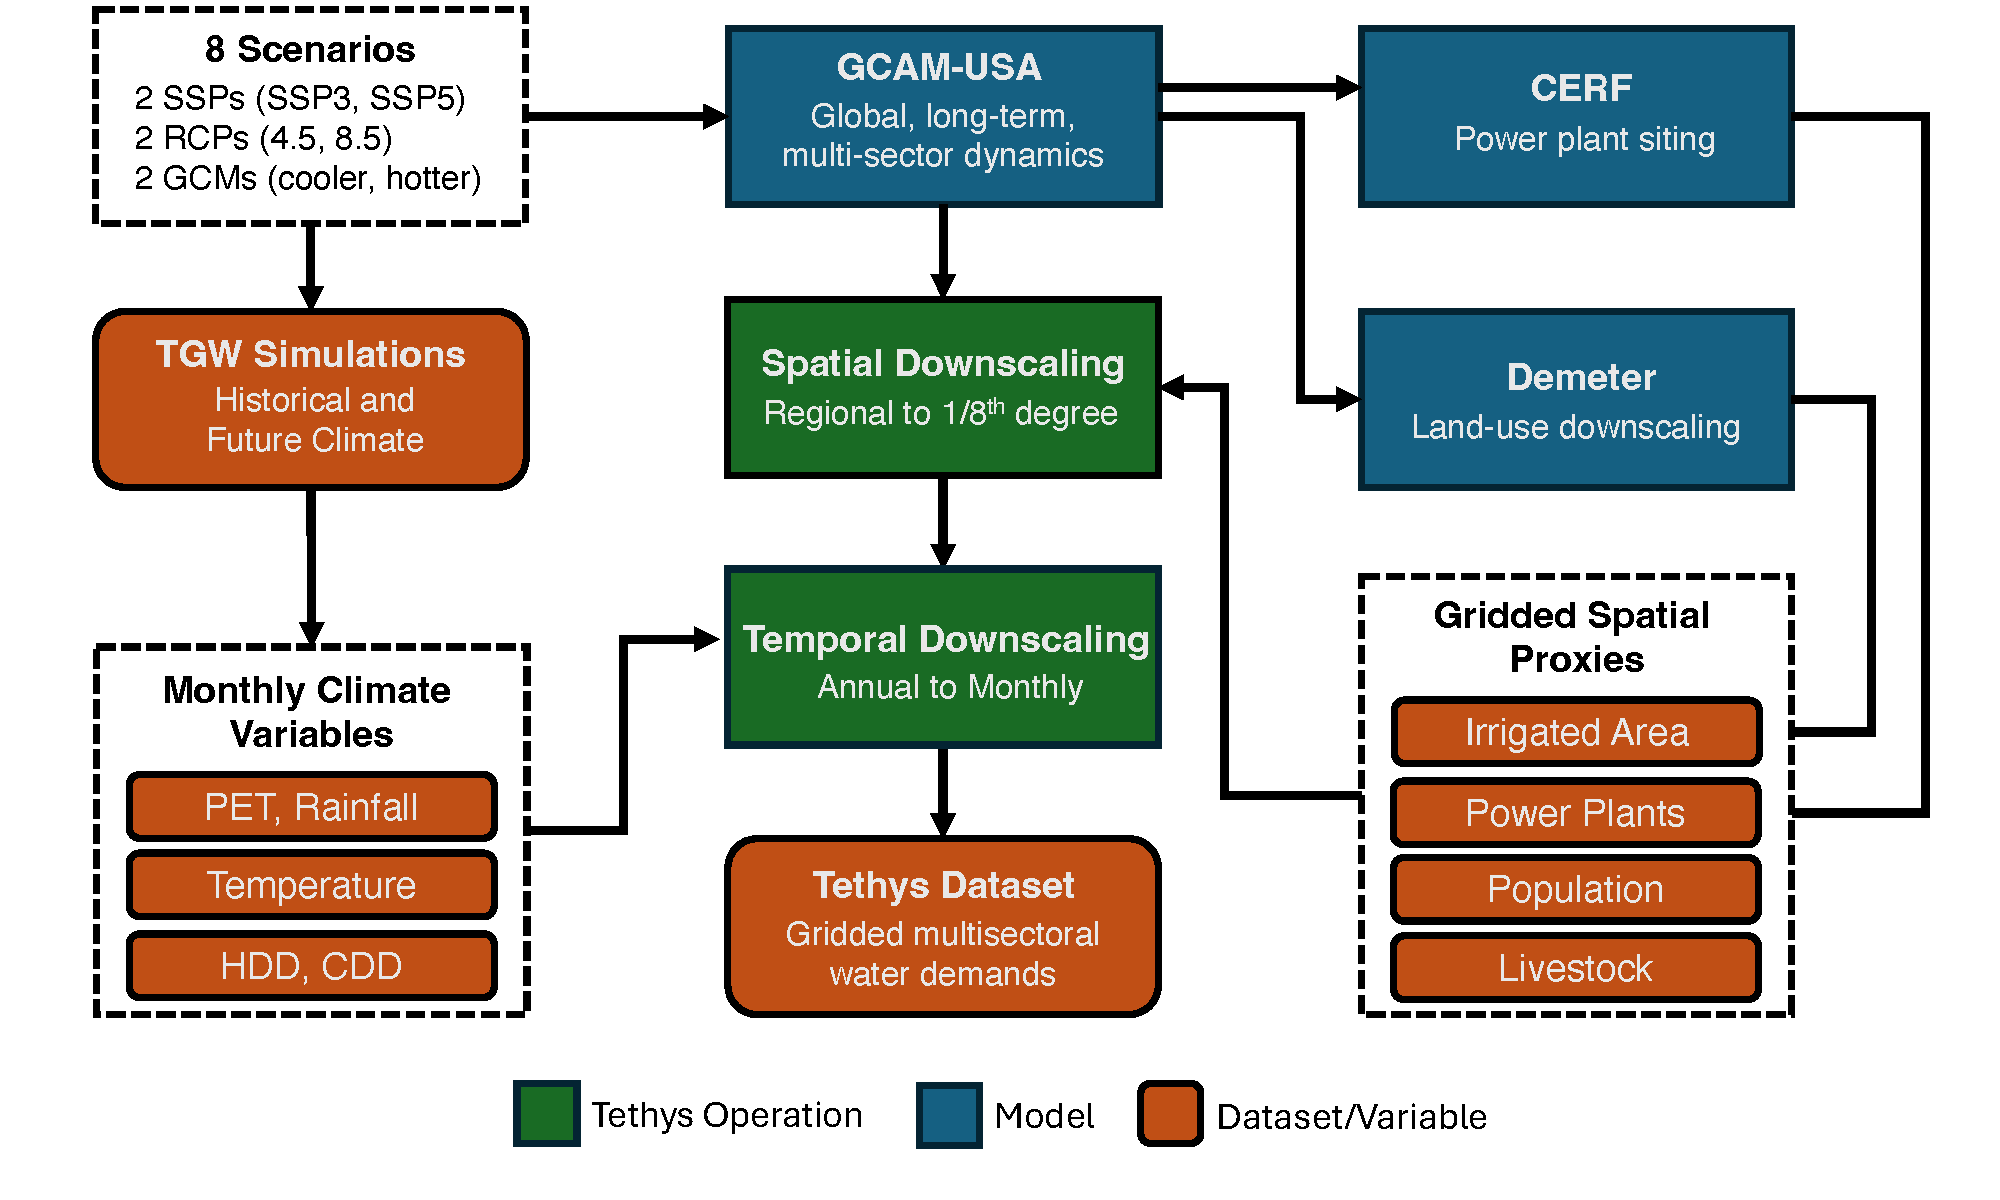
\includegraphics[width=0.85\linewidth]{flow-chart2.pdf}
%DIFDELCMD < %%%
\DIFdelendFL \DIFaddbeginFL \begin{tikzpicture}[
  font=\sffamily\small,
  node distance=8mm and 9mm,
  every node/.style={align=center},
  model/.style={
    draw, fill=blue!20!gray!70, text=white,
    rounded corners=1pt, minimum width=32mm, minimum height=12mm,
    inner sep=2pt
  },
  op/.style={
    draw, fill=olive!50!black!70, text=white,
    rounded corners=1pt, minimum width=42mm, minimum height=12mm,
    inner sep=2pt
  },
  data/.style={
    draw, fill=orange!60!brown!80, text=white,
    rounded corners=4pt, minimum width=32mm, minimum height=10mm,
    inner sep=2pt
  },
  groupbox/.style={
    draw, dashed, rounded corners=2pt, inner sep=4pt
  },
  tethysbox/.style={
    draw=olive!40!black, very thick, rounded corners=2pt, inner sep=6pt,
    fill=olive!20!black!5
  },
  arrow/.style={-{Latex[length=2mm]}, thick}
]

% --- Top row: scenarios -> GCAM-USA -> CERF
\node[op, fill=none, draw=none, text=black] (scenariobox-anchor) {};
\node[draw, dashed, rounded corners=2pt, inner sep=6pt, minimum width=42mm,
      align=left] (scenariobox) at (0,0) {%
  \textbf{8 Scenarios}\\
  2 SSPs (SSP3, SSP5)\\
  2 RCPs (4.5, 8.5)\\
  2 GCMs (cooler, hotter)
};
\node[model, right=20mm of scenariobox, minimum width=42mm, minimum height=14mm] (gcam) {%
  \textbf{GCAM-USA}\\[1pt]
  Global, long-term,\\
  multi-sector dynamics
};
\node[model, right=10mm of gcam, minimum height=14mm] (cerf) {%
  \textbf{CERF}\\[1pt]
  Power plant siting
};

% --- Left column: TGW + monthly meteorological variables
\node[data, below=12mm of scenariobox, minimum width=42mm, minimum height=14mm] (tgw) {%
  \textbf{TGW Simulations}\\
  Historical and\\
  Future Climate
};
\node[draw, dashed, rounded corners=2pt, inner sep=4pt, below=8mm of tgw,
      minimum width=42mm, align=center] (metbox) {%
  \textbf{Monthly Meteorological Variables}\\[2pt]
  \begin{tikzpicture}[baseline=(c.base)]
    \node[data, minimum width=34mm, minimum height=6mm] (m1) {PET, Rainfall};
    \node[data, below=1.5mm of m1, minimum width=34mm, minimum height=6mm] (m2) {Temperature};
    \node[data, below=1.5mm of m2, minimum width=34mm, minimum height=6mm] (c) {HDD, CDD};
  }
\end{tikzpicture}\DIFaddFL{;
}

%DIF >  --- Center column: Tethys wrapper around Spatial + Temporal Downscaling
\node[op, below=12mm of gcam, minimum width=46mm] \DIFaddFL{(spatial) }{%DIF > 
  \textbf{\DIFaddFL{Spatial Downscaling}}\\
  \DIFaddFL{Regional to 1/8$^{\circ}$
}}\DIFaddFL{;
}\node[op, below=8mm of spatial, minimum width=46mm] \DIFaddFL{(temporal) }{%DIF > 
  \textbf{\DIFaddFL{Temporal Downscaling}}\\
  \DIFaddFL{5-year to monthly
}}\DIFaddFL{;
}\begin{scope}[on background layer]
\node[tethysbox, fit=(spatial)(temporal), label={[anchor=north west, font=\sffamily\bfseries]north west:Tethys}] \DIFaddFL{(tethys) }{}\DIFaddFL{;
}\end{scope}

%DIF >  --- Output
\node[data, below=10mm of temporal, minimum width=46mm, minimum height=12mm] \DIFaddFL{(out) }{%DIF > 
  \textbf{\DIFaddFL{Tethys Dataset}}\\
  \DIFaddFL{Gridded multisectoral}\\
  \DIFaddFL{water demands
}}\DIFaddFL{;
}

%DIF >  --- Right column: Demeter + gridded spatial proxies
\node[model, below=8mm of cerf, minimum width=46mm, minimum height=18mm, align=center] \DIFaddFL{(demeter) }{%DIF > 
  \textbf{\DIFaddFL{Demeter}}\\[1pt]
  \DIFaddFL{Land-use downscaling}\\
  \scriptsize \DIFaddFL{regional 5-yr $\to$ 1/8$^{\circ}$ annual
}}\DIFaddFL{;
}\node[draw, dashed, rounded corners=2pt, inner sep=4pt, below=14mm of demeter,
      align=center] \DIFaddFL{(proxybox) }{%DIF > 
  \textbf{\DIFaddFL{Gridded Spatial Proxies}}\\[2pt]
  \begin{tikzpicture}[baseline=(p4.base)]
    \node[data, minimum width=34mm, minimum height=6mm] (p1) {Irrigated Area};
    \node[data, below=1.5mm of p1, minimum width=34mm, minimum height=6mm] (p2) {Power Plants};
    \node[data, below=1.5mm of p2, minimum width=34mm, minimum height=6mm] (p3) {Population};
    \node[data, below=1.5mm of p3, minimum width=34mm, minimum height=6mm] (p4) {Livestock};
  \end{tikzpicture}
}\DIFaddFL{;
}

%DIF >  --- Connecting arrows
\draw[arrow] \DIFaddFL{(scenariobox.east) -- (gcam.west);
}\draw[arrow] \DIFaddFL{(gcam.east) -- (cerf.west);
}\draw[arrow] \DIFaddFL{(gcam.south) -- (spatial.north);
}\draw[arrow] \DIFaddFL{(cerf.south) -- (demeter.north);
}\draw[arrow] \DIFaddFL{(gcam.south east) to}[\DIFaddFL{bend left=10}] \DIFaddFL{(demeter.north west);
}\draw[arrow] \DIFaddFL{(scenariobox.south) -- (tgw.north);
}\draw[arrow] \DIFaddFL{(tgw.south) -- (metbox.north);
}\draw[arrow] \DIFaddFL{(metbox.east) -- (temporal.west);
}\draw[arrow] \DIFaddFL{(proxybox.west) -- (spatial.east);
}\draw[arrow] \DIFaddFL{(cerf.south) -- ++(0,-2mm) -| (proxybox.north);
}\draw[arrow] \DIFaddFL{(demeter.south) -- (proxybox.north);
}\draw[arrow] \DIFaddFL{(spatial.south) -- (temporal.north);
}\draw[arrow] \DIFaddFL{(temporal.south) -- (out.north);
}

%DIF >  --- Legend
\node[draw, rounded corners=1pt, fill=olive!50!black!70, text=white,
      minimum width=22mm, minimum height=4mm,
      below=18mm of out, anchor=east, xshift=-2mm] \DIFaddFL{(legop) }{\DIFaddFL{Tethys Operation}}\DIFaddFL{;
}\node[draw, rounded corners=1pt, fill=blue!20!gray!70, text=white,
      minimum width=22mm, minimum height=4mm,
      right=2mm of legop] \DIFaddFL{(legmodel) }{\DIFaddFL{Model}}\DIFaddFL{;
}\node[draw, rounded corners=4pt, fill=orange!60!brown!80, text=white,
      minimum width=22mm, minimum height=4mm,
      right=2mm of legmodel] \DIFaddFL{(legdata) }{\DIFaddFL{Dataset/Variable}}\DIFaddFL{;
}

\end{tikzpicture}
\DIFaddendFL \caption{Workflow for producing the Tethys CONUS multi-sector water-demand dataset. \DIFdelbeginFL \DIFdelFL{State- }\DIFdelendFL \DIFaddbeginFL \DIFaddFL{Eight scenarios cross two SSPs, two RCPs, }\DIFaddendFL and \DIFdelbeginFL \DIFdelFL{HUC2-basin-scale demands from GCAM-USA }\DIFdelendFL \DIFaddbeginFL \DIFaddFL{two GCM-temperature samples }\DIFaddendFL (\DIFdelbeginFL \DIFdelFL{Section ``}\DIFdelendFL \DIFaddbeginFL \DIFaddFL{cooler/hotter). Each scenario drives }\DIFaddendFL GCAM-USA \DIFaddbeginFL \DIFaddFL{(}\DIFaddendFL regional \DIFdelbeginFL \DIFdelFL{projections''}\DIFdelendFL \DIFaddbeginFL \DIFaddFL{sectoral demands at the state/basin scale}\DIFaddendFL ) \DIFdelbeginFL \DIFdelFL{are spatially downscaled using sector-specific }\DIFdelendFL \DIFaddbeginFL \DIFaddFL{and TGW-WRF dynamical-downscaling simulations. Tethys (heavy outline) carries out the two downscaling operations: spatial downscaling from regional aggregates to the 1/8$^{\circ}$ CONUS grid, and temporal downscaling of the 5-year GCAM-USA outputs to monthly resolution. Spatial downscaling uses }\DIFaddendFL gridded proxies \DIFdelbeginFL \DIFdelFL{--- }\DIFdelendFL \DIFaddbeginFL \DIFaddFL{derived from }\DIFaddendFL Demeter \DIFaddbeginFL \DIFaddFL{(}\DIFaddendFL land use\DIFdelbeginFL \DIFdelFL{(Section ``Land-use projections (Demeter}\DIFdelendFL \DIFaddbeginFL \DIFaddFL{, regional 5-year $\to$ 1/8$^{\circ}$ annual}\DIFaddendFL )\DIFdelbeginFL \DIFdelFL{'')}\DIFdelendFL , CERF \DIFdelbeginFL \DIFdelFL{power-plant locations }\DIFdelendFL (\DIFdelbeginFL \DIFdelFL{Section ``Power-plant }\DIFdelendFL \DIFaddbeginFL \DIFaddFL{projected power-plant }\DIFaddendFL siting\DIFdelbeginFL \DIFdelFL{projections (CERF}\DIFdelendFL )\DIFdelbeginFL \DIFdelFL{'')}\DIFdelendFL , Jones and O'Neill \DIFaddbeginFL \DIFaddFL{(}\DIFaddendFL SSP-consistent \DIFdelbeginFL \DIFdelFL{gridded }\DIFdelendFL population\DIFaddbeginFL \DIFaddFL{)}\DIFaddendFL , and \DIFdelbeginFL \DIFdelFL{fixed }\DIFdelendFL GLW~3 \DIFdelbeginFL \DIFdelFL{livestock distributions }\DIFdelendFL (\DIFdelbeginFL \DIFdelFL{all in Section ``Spatial downscaling''}\DIFdelendFL \DIFaddbeginFL \DIFaddFL{livestock}\DIFaddendFL )\DIFdelbeginFL \DIFdelFL{. They are temporally downscaled using }\DIFdelendFL \DIFaddbeginFL \DIFaddFL{; temporal downscaling uses }\DIFaddendFL monthly meteorological variables --- potential evapotranspiration (PET), \DIFdelbeginFL \DIFdelFL{heating- and cooling-degree }\DIFdelendFL \DIFaddbeginFL \DIFaddFL{precipitation, mean temperature, heating degree }\DIFaddendFL days (HDD\DIFdelbeginFL \DIFdelFL{/}\DIFdelendFL \DIFaddbeginFL \DIFaddFL{), cooling degree days (}\DIFaddendFL CDD), and growing-season index (GSI) --- derived from \DIFdelbeginFL \DIFdelFL{the }\DIFdelendFL TGW-WRF\DIFdelbeginFL \DIFdelFL{meteorological dataset (Section ``Meteorological forcing (TGW-WRF)''), and post-processed with USGS-anchored adjustment of per-cell renewable vs}\DIFdelendFL .\DIFdelbeginFL \DIFdelFL{\ non-renewable source shares (Section ``Renewable vs.\ non-renewable source-share post-processing'').}\DIFdelendFL }
\label{fig:schematic}
\end{figure}

\begin{table}[ht]
\centering
\small
\begin{tabular}{lllll}
\toprule
\textbf{Dataset} & \textbf{Spatial res.} & \textbf{Temporal res.} & \textbf{Scenarios} & \textbf{Sectors} \\
\midrule
Huang et al.\cite{Huang2018}                   & 0.5$^{\circ}$ global & monthly & historical (1971--2010) & 6 sectors \\
Khan et al.\cite{Khan2023} (prior Tethys)      & 0.5$^{\circ}$ global & monthly & historical + SSP/RCP futures & 6 sectors \\
van Vliet et al.\cite{van_Vliet_2021}          & country/basin & annual & historical + SSP & 6 sectors \\
Wada et al.\cite{Wada_2017}                    & 0.5$^{\circ}$ global & monthly & historical + projections & 4 sectors \\
\textbf{This work}                             & \textbf{0.125$^{\circ}$ CONUS} & \textbf{monthly} & \textbf{hist.\ + 8 RCP/climate/SSP} & \textbf{6 sectors + GW/SW split} \\
\bottomrule
\end{tabular}
\caption{Gridded multi-sector water-demand datasets that overlap in scope with the product presented here. The current dataset increases spatial resolution fourfold over its immediate Tethys predecessor\cite{Khan2023}, adds per-cell groundwater/surface-water attribution, and uses scenario-consistent population, land-use, and climate forcing rather than static baselines.}
\label{tab:prior-datasets}
\end{table}

% -----------------------------------------------------------------------------
\section*{Methods and Data}

The Tethys downscaling chain (Figure~\ref{fig:schematic}) converts state- and basin-scale water-demand projections from GCAM-USA into 1/8$^{\circ}$ monthly gridded fields by applying sector-specific spatial proxies (land use, power-plant siting, population, livestock, derived from Demeter, CERF, the Jones \& O'Neill SSPs, and GLW~3, respectively), distributing the annual values into months using TGW-WRF derived meteorological indicators (deficit, growing-season index, heating- and cooling-degree-days), and finally adjusting each cell's renewable-vs.-non-renewable share against USGS observations. The remainder of this section is organized in two parts. The first part describes the exogenous scenarios and inputs to Tethys: the eight-scenario factorial, the TGW meteorological forcing, GCAM-USA, the Demeter land-use projections, and the CERF power-plant projections. The second part describes the Tethys mechanics: the spatial-downscaling step (Eq.~\ref{eq:spatial}) with sector-specific proxies, the temporal-downscaling step with sector-specific monthly weights, and the source-share post-processing (Eq.~\ref{eq:source-shares}). The closing subsection documents the modular-coupling design.

\subsection*{Scenarios}

The dataset spans one historical period (1980--2019) and an eight-scenario factorial of futures (2020--2100), constructed jointly with the IM3/GCIMS framework\cite{Mongird2025CERF}. The factorial crosses three two-level dimensions: emissions constraints (rcp45 = moderate constraints, rcp85 = no constraints), GCM-temperature sensitivity over CONUS (cooler vs.\ hotter CMIP6 model groups), and Shared Socioeconomic Pathway (SSP3 = low population/economic growth, SSP5 = high). Following the IM3 ScenarioMIP convention, we use the acronym ``rcp'' for brevity in scenario names, although the underlying perturbed-thermodynamics simulations are derived from CMIP6, not CMIP5\cite{Mongird2025CERF}. The eight scenario directory names (e.g., \texttt{rcp45cooler\_ssp3}) appear in Table~\ref{tab:scenarios} and the inter-scenario behavio\DIFaddbegin \DIFadd{u}\DIFaddend r of CONUS demand is shown in Figure~\ref{fig:scenarios}.

\subsection*{Meteorological forcing (TGW-WRF)}

The Thermodynamic Global Warming (TGW) meteorological forcing\cite{Jones2023TGW} provides hourly atmospheric variables at 1/8$^{\circ}$ over CONUS, dynamically downscaled with WRF from a 30-km ERA5 historical baseline (1980--2019) and from CMIP6-derived monthly thermodynamic perturbations (2020--2100). The TGW approach replays historical weather sequences with added thermodynamic signals, retaining the synoptic structure of observed weather while shifting its mean state to match each future scenario. For each TGW scenario we compute daily potential evapotranspiration (PET), precipitation ($P$), mean temperature, heating degree days (HDD), cooling degree days (CDD), and a growing-season index (GSI). These are aggregated to monthly totals or means and reprojected to the Tethys 1/8$^{\circ}$ CONUS grid.

The monthly water deficit used in irrigation temporal downscaling is $\Delta_m = \max\!\big(\text{PET}_m - P_m,\, 0\big)$. The monthly GSI is derived from a simplified version of Jolly et al.\cite{Jolly_2005}, retaining the daily minimum-temperature and daylength indicators but omitting the vapour-pressure-deficit term. For each day $d$,
\begin{equation}
f(T_{\min,d}) = \min\!\left(\max\!\left(\frac{T_{\min,d}+2}{7},\,0\right),\,1\right), \qquad
g(L_d) = \min\!\left(\max\!\left(L_d - 10,\,0\right),\,1\right),
\label{eq:gsi-components}
\end{equation}
where $T_{\min,d}$ is the daily minimum air temperature (\textdegree C) and $L_d$ is the daylength (hours). Monthly GSI is the daily-mean product over month $m$,
\begin{equation}
G_m = \big\langle f(T_{\min,d}) \cdot g(L_d) \big\rangle_{d \in m}.
\label{eq:gsi-monthly}
\end{equation}
Preprocessing code is archived under \texttt{scripts/0\_preprocessing/gsi\_nersc/} in the integration meta-repository (see Code availability).

\subsection*{GCAM-USA regional projections}

Region-scale water-demand inputs come from the Global Change Analysis Model (GCAM-USA version)\cite{Zhao_gcamusa_water,Zhao2024,Calvin2019GCAM,Binsted_2022}. GCAM is a market-equilibrium integrated assessment model that allocates supply and demand across coupled energy, water, land, and economic sectors under scenario-specific assumptions on population, productivity, technology, and policy. GCAM-USA resolves U.S.\ electricity generation, manufacturing, and municipal demands at the state level and crop-level irrigation demands at state \DIFdelbegin \DIFdel{/}\DIFdelend \DIFaddbegin \DIFadd{$\times$ }\DIFaddend basin intersections, at 5-year intervals. Each of the eight runs corresponds to one cell of the scenario factorial; we refer readers to Mongird et al.\cite{Mongird2025CERF} for the full energy-water-land coupling description and limit ourselves here to how the GCAM-USA outputs feed the Tethys workflow of Figure~\ref{fig:schematic}.

\subsection*{Land-use projections (Demeter)}

Spatially explicit, scenario-consistent annual per-crop irrigated-area maps at 1/8$^{\circ}$ come from Demeter\cite{Vernon-2018}, a land-use spatial disaggregation model that reconciles a high-resolution land-use baseline with GCAM regional boundary conditions using transition-priority rules that distinguish intensification (increase of a land type within a cell) from extensification (spread from an adjacent cell). For irrigation, Demeter outputs cover the 13 crop classes that GCAM-USA reports (Corn, Wheat, Rice, RootTuber, OilCrop, SugarCrop, OtherGrain, FiberCrop, FodderGrass, FodderHerb, biomass, MiscCrop, PalmFruit). The per-crop irrigated-area fields serve as the spatial proxy for irrigation in the Tethys spatial-downscaling step (below).

\subsection*{Power-plant siting projections (CERF)}

Future thermoelectric capacity is sited at $\approx$1-km resolution by the Capacity Expansion Regional Feasibility (CERF) model\cite{Vernon2021,Mongird2025CERF}, which places projected plants based on siting feasibility (exclusion layers, transmission proximity, cooling-water access) and locational economics, conditional on the GCAM-USA state-level capacity trajectory for each scenario. Plants represent thermoelectric generation (coal, natural gas, oil, nuclear, biomass, geothermal, concentrated solar thermal), excluding hydropower. CERF-sited plants are aggregated to 1/8$^{\circ}$ grid cells, and the cell-level installed capacity (MW) serves as the spatial proxy for thermoelectric demand. For the historical period we substitute the 2015 plant inventory from the Global Power Plant Database v1.3 (GPPD), augmented with the IM3 experiment B CONUS plant inventory, in place of CERF projections; both feed the same spatial-downscaling step at the cell.

\subsection*{Spatial downscaling}

We assume that the location of demand within a region follows a gridded proxy appropriate to the sector. For any sector with total demand $D_{\mathrm{region}}$ and proxy field $\pi_{\mathrm{cell}}$,
\begin{equation}
D_{\mathrm{cell}} = D_{\mathrm{region}} \times \frac{\pi_{\mathrm{cell}}}{\sum_{c \in \mathrm{region}} \pi_{c}}.
\label{eq:spatial}
\end{equation}
For irrigation, the proxy is per-crop irrigated area from Demeter (above). For thermoelectric, the proxy is CERF-sited installed capacity (above). For municipal demand, we use the SSP-consistent Jones and O'Neill\cite{Jones_2016} gridded population at 10-year intervals, linearly interpolating between bracketing decadal maps, with state-level GCAM-USA municipal demand allocated to cells in proportion to projected population. For livestock, the proxy is the GLW~3 gridded head-count map\cite{Gilbert2018} at 1/12$^{\circ}$ for reference year 2010, re-gridded to 1/8$^{\circ}$ by area-overlap allocation and held fixed across all years and scenarios; livestock is \textasciitilde2\% of CONUS demand, so the static-distribution assumption has limited aggregate impact (see Limitations). The mapping from GCAM livestock sectors to GLW animals follows Table~\ref{tab:livestock}. For manufacturing and mining, we use population as the spatial proxy, following prior Tethys work\cite{Khan2023}.

\begin{table}[ht]
\centering
\begin{tabular}{ll}
\toprule
\textbf{GCAM livestock sector} & \textbf{GLW proxy animal(s)} \\
\midrule
Beef      & Buffalo + Cattle \\
Dairy     & Buffalo + Cattle \\
Pork      & Pig \\
Poultry   & Chicken + Duck \\
SheepGoat & Sheep + Goat \\
\bottomrule
\end{tabular}
\caption{Mapping from GCAM livestock sectors to animal species in the GLW~3 dataset.}
\label{tab:livestock}
\end{table}

\subsection*{Temporal downscaling}

GCAM-USA operates at 5-year steps. We linearly interpolate spatially-downscaled outputs to annual resolution and then distribute the annual demand at each cell into 12 monthly values using sector-specific formulas. For livestock, manufacturing, and mining we hold monthly demand uniform at $1/12$ of the annual total; irrigation, electricity, and domestic follow climate-driven formulations described next.

\subsubsection*{Irrigation}

For each cell and year, we compute a monthly weight field from the growing-season index $G_m$ (Eq.~\ref{eq:gsi-monthly}), the monthly deficit $\Delta_m$, and month length $N_m$:
\begin{equation}
\tilde{w}_m = \frac{\Delta_m \, G_m}{N_m}\quad, \qquad w_m = \frac{\tilde{w}_m}{\sum_{k=1}^{12}\tilde{w}_k},
\label{eq:irr-weights}
\end{equation}
so $\sum_m w_m = 1$ and monthly irrigation demand is $D_m = w_m \, D_{\mathrm{year}}$. Equation~(\ref{eq:irr-weights}) operationalizes the combined deficit-and-growing-season approach of Moore et al.\cite{Moore_2015} and Roy et al.\cite{Roy_2005}: water demand concentrates in months that are simultaneously water-limited ($\Delta_m > 0$) and vegetatively active ($G_m > 0$). The weights are per-cell and differ across cells and years.

\subsubsection*{Electricity}

We distribute monthly electricity water demand by splitting annual use into heating, cooling, and other shares, each weighted by an HDD/CDD-driven monthly profile. Region-level shares of annual electricity consumption for heating $p_{\mathrm{heat}}$, cooling $p_{\mathrm{cool}}$, and other $p_{\mathrm{other}}$ come from GCAM-USA. At each cell, define annual sums $H_y = \sum_m \text{HDD}_m$ and $C_y = \sum_m \text{CDD}_m$ and monthly distribution fields $\hat{h}_m$ and $\hat{c}_m$ with
\begin{equation}
(\hat{h}_m,\,\hat{c}_m) =
\begin{cases}
\big(\text{HDD}_m / H_y,\ \text{CDD}_m / C_y\big)      & H_y \ge 650 \text{ and } C_y \ge 450 \\[2pt]
\big(\text{HDD}_m / H_y,\ \text{HDD}_m / H_y\big)      & H_y \ge 650 \text{ and } C_y < 450 \\[2pt]
\big(\text{CDD}_m / C_y,\ \text{CDD}_m / C_y\big)      & H_y < 650 \text{ and } C_y \ge 450 \\[2pt]
(1/12,\ 1/12)                                          & H_y < 650 \text{ and } C_y < 450,
\end{cases}
\label{eq:elec-cases}
\end{equation}
with $\hat{o}_m = 1/12$ always. Monthly demand is
\begin{equation}
D_m = D_{\mathrm{year}} \times \big(p_{\mathrm{heat}}\,\hat{h}_m + p_{\mathrm{cool}}\,\hat{c}_m + p_{\mathrm{other}}\,\hat{o}_m\big).
\label{eq:elec-demand}
\end{equation}
The first case applies to cells with both a meaningful heating season (annual HDD $\ge 650$) and a meaningful cooling season (annual CDD $\ge 450$). The second and third cases collapse onto whichever signal is non-trivial, preventing division by near-zero annual sums in climates dominated by one extreme. The fourth case reverts to a uniform distribution where neither threshold is exceeded. The threshold convention follows Huang et al.\cite{Huang2018}.

\subsubsection*{Domestic}

For the domestic (residential public-supply) sector we use the temperature-anomaly formula of Wada et al.\cite{Wada2011}:
\begin{equation}
D_m = \frac{D_{\mathrm{year}}}{12} \times \left(\frac{T_m - \bar{T}}{T_{\max} - T_{\min}}\,R + 1\right),
\label{eq:dom-monthly}
\end{equation}
where $T_m$ is the monthly mean temperature at the cell, $\bar{T}$ is the annual mean temperature, $T_{\max}$ and $T_{\min}$ are the annual extremes, and $R$ is a region-scale amplitude coefficient drawn from a static regional map; higher $R$ implies stronger seasonal amplification. We clip negative values to zero so that $D_m \ge 0$ in every cell.

\subsection*{Renewable vs.\ non-renewable source-share post-processing}

GCAM-USA solves for the share of each basin's withdrawals met from renewable (surface) versus non-renewable (groundwater) supply by cost-based allocation. Mapping that basin-scale split onto the 1/8$^{\circ}$ grid requires two steps. First, we apply the basin-level share uniformly to all end-use sectors in the basin, except that thermoelectric demand is assumed to use surface water only and the remaining sectoral shares are renormalized accordingly. Second, we anchor the historical spatial pattern of the renewable/non-renewable mix to observed USGS data by rescaling each cell's GCAM share against its historical-2015 value while preserving the spatial pattern of a static USGS baseline derived from the 2009-2020 mean renewable/non-renewable share distribution. Let $s^{\mathrm{GCAM}}_{c,y}$ denote the GCAM-derived renewable share at cell $c$ in year $y$, and $s^{\mathrm{USGS}}_c$ the static USGS-derived baseline share at cell $c$. For the subset of cells $\mathcal{M}$ for which both $s^{\mathrm{GCAM}}_{c,\,2015}>0$ and $s^{\mathrm{USGS}}_c$ is available, the adjusted share is
\begin{equation}
s^{\mathrm{adj}}_{c,y} =
\begin{cases}
\displaystyle \min\!\left(1,\; s^{\mathrm{USGS}}_c \times \frac{s^{\mathrm{GCAM}}_{c,y}}{s^{\mathrm{GCAM}}_{c,\,2015}}\right) & c \in \mathcal{M} \\[10pt]
s^{\mathrm{GCAM}}_{c,y}                                                                                        & c \notin \mathcal{M}.
\end{cases}
\label{eq:source-shares}
\end{equation}
The $\min(\cdot,1)$ clip prevents amplifications when the 2015 GCAM baseline is small. In groundwater-dominated regions the clip can mask trajectory increases, but it preserves the physical bound that a share cannot exceed one. The USGS spatial pattern is anchored in place where observable, and the GCAM scenario trajectory enters only as a per-cell temporal ratio.

\subsection*{Modular earth system model coupling}

The dataset combines simulation outputs produced, in some cases, by independent teams that use consistent assumptions: the GCAM-USA run uses one scenario configuration for each SSP$\times$RCP combination; Demeter is run with the corresponding GCAM scenario to produce per-crop irrigated-area maps; CERF sites power plants using GCAM-USA state-level capacity trajectories; the Jones and O'Neill SSP3/SSP5 population maps are used as-is; and the TGW-WRF climate sample is drawn from a fixed ensemble conditioned on the RCP. We do not perfectly co-calibrate these inputs, which would be prohibitively expensive computationally; instead, we document the specific versions used (see Code availability) and treat the resulting record as scenario-plausible but not a single self-consistent Earth-system simulation. This modular ``frankenstein'' coupling is an established compromise in multi-sector dynamics modeling\cite{Khan2023} and is appropriate for a dataset intended to support sensitivity and adaptation studies, not causal attribution. The combined chain is scenarios $\to$ TGW-WRF forcing $\to$ GCAM-USA $\to$ Demeter/CERF/SSP-pop/GLW-3 spatial proxies $\to$ TGW-driven temporal weights $\to$ USGS-anchored source-share clip --- produces the 1/8$^{\circ}$ monthly gridded record described next.

% -----------------------------------------------------------------------------
\section*{Data Records}

The dataset is permanently archived and openly available on MSD-Live (\url{https://data.msdlive.org/uploads/p4xce-e8822}); the Tethys model source is at \href{https://github.com/JGCRI/tethys}{github.com/JGCRI/tethys}.

Scenario directories (Table~\ref{tab:scenarios}) each contain per-sector netCDF~4 files following the naming convention \texttt{<Sector>\_<demand\_type>[\_monthly].nc}. \texttt{<Sector>} is one of \{\texttt{Domestic}, \texttt{Electricity}, \texttt{Irrigation}, \texttt{Livestock}, \texttt{Manufacturing}, \texttt{Mining}\}, and \texttt{<demand\_type>} is \texttt{withdrawals} or \texttt{consumption}. The \texttt{\_monthly} suffix marks monthly files; for irrigation, the \texttt{\_with\_losses} suffix marks files that include conveyance losses.

Each scenario directory also contains \texttt{gridded\_runoff\_shares.nc} (per-year, per-cell renewable share $s^{\mathrm{adj}}_{c,y}$ from Eq.~\ref{eq:source-shares}, used to recover the surface/groundwater split of withdrawals) and two YAML configuration files (\texttt{config\_withdrawals.yaml}, \texttt{config\_consumption.yaml}) that record the exact Tethys run configuration used to produce the files. All sector files share the same \texttt{(year, lat, lon)} or \texttt{(year, lat, lon, month)} schema with sector-specific sub-variables; Figure~\ref{fig:data-listing} shows an example CDL listing. Table~\ref{tab:scenarios} enumerates the eight scenarios; the next section validates this published record against USGS observations.

% Need to revise this based on new runs
\begin{table}[ht]
\centering
\begin{tabular}{lll}
\toprule
\textbf{Scenario directory} & \textbf{Time span} & \textbf{Description} \\
\midrule
\texttt{historical}         & 1980--2019 & Observed-period baseline using historical climate and population. \\
\texttt{rcp45cooler\_ssp3}  & 2020--2100 & Lower-emissions, cooler TGW sample, SSP3 socioeconomics. \\
\texttt{rcp45cooler\_ssp5}  & 2020--2100 & Lower-emissions, cooler TGW sample, SSP5 socioeconomics. \\
\texttt{rcp45hotter\_ssp3}  & 2020--2100 & Lower-emissions, hotter TGW sample, SSP3. \\
\texttt{rcp45hotter\_ssp5}  & 2020--2100 & Lower-emissions, hotter TGW sample, SSP5. \\
\texttt{rcp85cooler\_ssp3}  & 2020--2100 & Higher-emissions, cooler TGW sample, SSP3. \\
\texttt{rcp85cooler\_ssp5}  & 2020--2100 & Higher-emissions, cooler TGW sample, SSP5. \\
\texttt{rcp85hotter\_ssp3}  & 2020--2100 & Higher-emissions, hotter TGW sample, SSP3. \\
\texttt{rcp85hotter\_ssp5}  & 2020--2100 & Higher-emissions, hotter TGW sample, SSP5. \\
\bottomrule
\end{tabular}
\caption{Scenario directories in the published dataset. Each directory contains per-sector withdrawal and consumption netCDFs, a gridded runoff-share file, and the two Tethys YAML configurations used to generate them.}
\label{tab:scenarios}
\end{table}

\begin{figure}[ht]
\centering
\begin{verbatim}
netcdf Livestock_withdrawals_monthly {
dimensions:
    year = 46 ;
    lat = 224 ;
    lon = 464 ;
    month = 12 ;
variables:
    float Beef(year, lat, lon, month) ;
    float Dairy(year, lat, lon, month) ;
    float Pork(year, lat, lon, month) ;
    float Poultry(year, lat, lon, month) ;
    float SheepGoat(year, lat, lon, month) ;
    double lat(lat) ;
    double lon(lon) ;
    int64 year(year) ;
    int64 month(month) ;
    int64 spatial_ref ;
}
\end{verbatim}
\caption{CDL excerpt of a monthly livestock-withdrawals netCDF. Other sectors share the same \texttt{(year, lat, lon [, month])} layout with sector-specific sub-variables.}
\label{fig:data-listing}
\end{figure}

% -----------------------------------------------------------------------------
\section*{Technical Validation}

We validate the downscaled dataset against USGS observations at the three sectors that together account for over 90\% of CONUS water demand: irrigation, thermoelectric, and domestic (public supply)\cite{skinnerWaterWithdrawalConsumption2025}. The goal is to establish that the downscaled record reproduces the dominant features of observed spatial and temporal demand patterns, with quantified bias where it departs --- not to declare a ``true'' dataset, since neither USGS nor Tethys is a direct observation at 1/8$^{\circ}$ resolution. Reference data are the USGS five-year water-use records, refreshed in January~2025, at the HUC12 scale for public supply and irrigation and per-plant for thermoelectric. We proceed from coarse to fine and from total to seasonal: CONUS annual totals, HUC6 spatial agreement and per-sector summary metrics, a bias-diagnosis subsection, the CONUS monthly cycle, and inter-scenario consistency.


\begin{table}[ht]
\centering
\begin{tabular}{lcccccc}
\toprule
\textbf{Sector} & \textbf{Pearson r} & \textbf{Spearman} & \textbf{NSE\DIFdelbeginFL \DIFdelFL{/KGE}\DIFdelendFL } & \textbf{MBE (\%)} & \textbf{NRMSE (\%)} & \textbf{MedAPE (\%)} \\
\midrule
\DIFdelbeginFL \DIFdelFL{Irrigation   }\DIFdelendFL \DIFaddbeginFL \DIFaddFL{Domestic     }\DIFaddendFL & 0.95 & \DIFdelbeginFL \DIFdelFL{0.92 }\DIFdelendFL \DIFaddbeginFL \DIFaddFL{0.97 }\DIFaddendFL & \DIFdelbeginFL \DIFdelFL{0.85 }\DIFdelendFL \DIFaddbeginFL \DIFaddFL{0.86 }\DIFaddendFL & \DIFdelbeginFL \DIFdelFL{+5   }\DIFdelendFL \DIFaddbeginFL \DIFaddFL{$+7$  }\DIFaddendFL & \DIFdelbeginFL \DIFdelFL{12 }\DIFdelendFL \DIFaddbeginFL \DIFaddFL{68  }\DIFaddendFL & \DIFdelbeginFL \DIFdelFL{8  }\DIFdelendFL \DIFaddbeginFL \DIFaddFL{37 }\DIFaddendFL \\
Electricity  & \DIFdelbeginFL \DIFdelFL{0.88 }\DIFdelendFL \DIFaddbeginFL \DIFaddFL{0.73 }\DIFaddendFL & \DIFdelbeginFL \DIFdelFL{0.85 }\DIFdelendFL \DIFaddbeginFL \DIFaddFL{0.78 }\DIFaddendFL & \DIFdelbeginFL \DIFdelFL{0.72 }\DIFdelendFL \DIFaddbeginFL \DIFaddFL{0.39 }\DIFaddendFL & \DIFdelbeginFL \DIFdelFL{-30  }\DIFdelendFL \DIFaddbeginFL \DIFaddFL{$-2$  }\DIFaddendFL & \DIFdelbeginFL \DIFdelFL{25 }\DIFdelendFL \DIFaddbeginFL \DIFaddFL{171 }\DIFaddendFL & \DIFdelbeginFL \DIFdelFL{15 }\DIFdelendFL \DIFaddbeginFL \DIFaddFL{86 }\DIFaddendFL \\
\DIFdelbeginFL \DIFdelFL{Domestic     }\DIFdelendFL \DIFaddbeginFL \DIFaddFL{Irrigation   }\DIFaddendFL & \DIFdelbeginFL \DIFdelFL{0.71 }\DIFdelendFL \DIFaddbeginFL \DIFaddFL{0.89 }\DIFaddendFL & \DIFdelbeginFL \DIFdelFL{0.68 }\DIFdelendFL \DIFaddbeginFL \DIFaddFL{0.80 }\DIFaddendFL & \DIFdelbeginFL \DIFdelFL{0.45 }\DIFdelendFL \DIFaddbeginFL \DIFaddFL{0.77 }\DIFaddendFL & \DIFdelbeginFL \DIFdelFL{-45  }\DIFdelendFL \DIFaddbeginFL \DIFaddFL{$-2$  }\DIFaddendFL & \DIFdelbeginFL \DIFdelFL{35 }\DIFdelendFL \DIFaddbeginFL \DIFaddFL{130 }\DIFaddendFL & \DIFdelbeginFL \DIFdelFL{22 }\DIFdelendFL \DIFaddbeginFL \DIFaddFL{79 }\DIFaddendFL \\
\bottomrule
\end{tabular}
\caption{Validation metrics for \DIFaddbeginFL \DIFaddFL{withdrawals in }\DIFaddendFL the three sectors that together account for over 90\% of CONUS water demand, against USGS \DIFdelbeginFL \DIFdelFL{2015 estimates }\DIFdelendFL \DIFaddbeginFL \DIFaddFL{five-year water-use records (2010--2020) }\DIFaddendFL at the HUC6 scale (\DIFdelbeginFL \DIFdelFL{$n=208$}\DIFdelendFL \DIFaddbeginFL \DIFaddFL{$n=329$ HUC6 basins for Domestic, $n=230$ for Electricity, $n=297$ for Irrigation; differences reflect basins where USGS reports zero use for that sector}\DIFaddendFL ). Metrics \DIFaddbeginFL \DIFaddFL{are computed on per-HUC6 means: USGS monthly demand summed to annual at each HUC6 and averaged across reporting years, compared against the matching Tethys aggregate. Domestic USGS values are scaled by 1.12 to align with the public-supply-only definition introduced after 2015~}\cite{skinnerWaterWithdrawalConsumption2025}\DIFaddFL{. Reported metrics }\DIFaddendFL include Pearson and Spearman correlations, Nash--Sutcliffe Efficiency (NSE)\DIFdelbeginFL \DIFdelFL{or Kling--Gupta Efficiency (KGE)}\DIFdelendFL , Mean Bias Error (MBE), Normalized Root Mean Square Error (NRMSE), and Median Absolute Percent Error (MedAPE). Values are computed by \DIFdelbeginFL \DIFdelFL{the validation pipeline at }\texttt{\DIFdelFL{tethys\_integration\_metarepo/validation/}}%DIFAUXCMD
\DIFdelendFL \DIFaddbeginFL \texttt{\DIFaddFL{tethys\_integration\_metarepo/validation/compute-table2-metrics.py}}\DIFaddendFL ; \DIFaddbeginFL \DIFaddFL{numerical outputs are shipped at }\texttt{\DIFaddFL{figures/validation-metrics.csv}}\DIFaddFL{. }\DIFaddendFL Livestock, Manufacturing, and Mining are not validated against USGS at HUC6 because they rely on static or population-proxy spatial allocation (see Limitations).}
\label{tab:validation-metrics}
\end{table}
\subsection*{CONUS annual totals}

Figure~\ref{fig:annual-total-timeseries} compares CONUS-aggregated annual demand for each of the three sectors and their sum. Tethys reproduces the magnitude of USGS CONUS totals within \DIFdelbegin \DIFdel{$\sim$}\DIFdelend \DIFaddbegin \DIFadd{roughly }\DIFaddend 10\% at annual resolution and follows the long-term trend (Table~\ref{tab:validation-metrics}\DIFaddbegin \DIFadd{, MBE within $\pm 7\%$ for all three sectors}\DIFaddend ). Magnitudes differ sharply across sectors, as expected: irrigation dominates consumptive use, while thermoelectric and irrigation withdrawals are of comparable magnitude. The decline in Electricity withdrawals reflects a known trend driven largely by the switch from coal-fired plants to other technologies\cite{skinnerWaterWithdrawalConsumption2025}. Figure~\ref{fig:annual-total-boxplot} shows the distribution of percent difference between the two records across HUC6 regions\DIFdelbegin \DIFdel{. Domestic shows the dominant negative bias at HUC6, partially offset at the CONUS total by the small positive bias in Irrigation; Electricity also runs negative}\DIFdelend \DIFaddbegin \DIFadd{; the within-basin spread is wide (NRMSE 68--171\% across sectors) even where the CONUS aggregate matches, reflecting compensating per-basin biases}\DIFaddend . The GCAM-USA 5-year time step manifests in Tethys annual irrigation demands as reduced interannual variability relative to USGS, which we promote to a Limitation.

\begin{figure}[ht]
\centering

\includegraphics[width=\linewidth]{val1-huc06-usgs-tethys-annual-total.png}
\caption{CONUS annual water use by sector from Tethys (black) and USGS (orange), 2000--2020.}
\label{fig:annual-total-timeseries}
\end{figure}

\begin{figure}[ht]
\centering

\includegraphics[width=\linewidth]{val2-huc06-usgs-tethys-annual-total-pdiff.png}
\caption{Percent difference between Tethys and USGS annual water use across HUC6 regions (\DIFdelbeginFL \DIFdelFL{n = 208}\DIFdelendFL \DIFaddbeginFL \DIFaddFL{$n=329$ basins for Domestic, 230 for Electricity, 297 for Irrigation}\DIFaddendFL ), by sector and demand type. Boxplot whiskers represent 1.5 times the interquartile range (IQR).}
\label{fig:annual-total-boxplot}
\end{figure}

\subsection*{HUC6 spatial agreement}

Figure~\ref{fig:map-pbias} maps the percent difference in annual average use at HUC6 scale. Tethys tends to exceed USGS in the Electricity sector, especially in the eastern and southeastern U.S.~where CERF-sited plants concentrate cooling demand in basins where USGS reports lower per-HUC totals. Tethys falls below USGS in Irrigation in several western basins --- notably the lower Colorado and parts of the Central Valley --- where the GSI-weighted monthly distribution underweights months that USGS records as heavy irrigation under observed 2015 conditions. At basin-wise correlation (Figure~\ref{fig:huc-correlation}), annual-average agreement at HUC6 \DIFdelbegin \DIFdel{ranges from 0.71 (Domestic ) to 0.95 (Irrigation), which we take as evidence that }\DIFdelend \DIFaddbegin \DIFadd{is strongest in Domestic ($r=0.95$), intermediate in Irrigation ($r=0.89$), and weakest in Electricity ($r=0.73$); }\DIFaddend the spatial pattern of use is \DIFdelbegin \DIFdel{well captured even where the magnitude is biased}\DIFdelend \DIFaddbegin \DIFadd{captured well even where individual basins carry magnitude bias}\DIFaddend .

\begin{figure}[ht]
\centering

\includegraphics[width=\linewidth]{val3-huc06-pdiff-usgs-tethys.png}
\caption{Percent difference in annual-average HUC6 water use, Tethys minus USGS, for Domestic, Electricity, and Irrigation sectors.}
\label{fig:map-pbias}
\end{figure}

\begin{figure}[ht]
\centering

\includegraphics[width=\linewidth]{val4-huc06-scatter-usgs-tethys.png}
\caption{HUC6 annual average demand, Tethys versus USGS, by sector and demand type. Pearson correlations\DIFdelbeginFL \DIFdelFL{range from 0.71 }\DIFdelendFL \DIFaddbeginFL \DIFaddFL{: 0.95 }\DIFaddendFL (Domestic)\DIFdelbeginFL \DIFdelFL{to 0.95 }\DIFdelendFL \DIFaddbeginFL \DIFaddFL{, 0.73 }\DIFaddendFL (\DIFaddbeginFL \DIFaddFL{Electricity), 0.89 (}\DIFaddendFL Irrigation)\DIFaddbeginFL \DIFaddFL{, computed on per-HUC6 means across the USGS reporting years 2010--2020}\DIFaddendFL .\DIFdelbeginFL \DIFdelFL{n = 208 HUC6 regions.}\DIFdelendFL }
\label{fig:huc-correlation}
\end{figure}

\subsection*{Bias diagnosis and uncertainty}

The \DIFdelbegin \DIFdel{$-45\%$ bias observed in Domestic demand (}\DIFdelend \DIFaddbegin \DIFadd{mean bias error (MBE) is small in aggregate (within $\pm 7\%$ for all three sectors at HUC6, }\DIFaddend Table~\ref{tab:validation-metrics})\DIFdelbegin \DIFdel{is }\DIFdelend \DIFaddbegin \DIFadd{, but the residual NRMSE and MedAPE remain large because per-basin biases compensate. The dominant per-basin pattern is a Domestic over-prediction in many basins ($\text{MedAPE} \approx 37\%$, modest aggregate $+7\%$ MBE after the public-supply 1.12 scaling), }\DIFaddend most likely attributable to the calibration of the Wada\cite{Wada2011} $R$ amplitude coefficient in Eq.~(\ref{eq:dom-monthly}), which was fit to aggregate USGS demand and may not capture the post-2015 public-supply subset, and to a mismatch in the GCAM-USA base-year socioeconomic data relative to USGS 2015 reporting. \DIFdelbegin \DIFdel{The $-30\%$ bias in Electricity withdrawals reflects two compounding factors}\DIFdelend \DIFaddbegin \DIFadd{Electricity has the lowest spatial agreement ($r=0.73$, Table~\ref{tab:validation-metrics}) and the largest within-basin spread (NRMSE $\approx 171\%$, MedAPE $\approx 86\%$)}\DIFaddend : GCAM-USA represents thermoelectric water use at state aggregates that already trail observed plant-by-plant cooling-water reductions over 2010--2015, and the CERF-sited capacity proxy concentrates demand at projected build-out locations rather than at the historical plant locations USGS observes\DIFdelbegin \DIFdel{. The $+5\%$ bias in Irrigation is small and not separately diagnosed}\DIFdelend \DIFaddbegin \DIFadd{, which produces the basin-by-basin scatter visible in Figure~\ref{fig:annual-total-boxplot}. Irrigation tracks USGS most closely in aggregate ($\text{MBE} \approx -2\%$) but with comparable per-basin spread (NRMSE $\approx 130\%$, MedAPE $\approx 79\%$), driven by the western-basin underweighting visible in Figure~\ref{fig:map-pbias}}\DIFaddend . Reference USGS estimates themselves carry inherent uncertainties, particularly in the thermoelectric and irrigation sectors, as documented in recent reanalyses\cite{Harris2025, Stets2025USGS}.

\subsection*{Seasonal cycle}

Figure~\ref{fig:monthly} compares the mean monthly cycle at CONUS scale. Irrigation and Electricity withdrawals reproduce the seasonal shape observed by USGS closely. Electricity consumption shows a consistent low offset in non-summer months, likely from the GCAM-USA representation of non-cooling electricity water use. Domestic shows the \DIFdelbegin \DIFdel{consistent negative bias also }\DIFdelend \DIFaddbegin \DIFadd{small positive aggregate bias }\DIFaddend seen in the annual MBE (Table~\ref{tab:validation-metrics}\DIFaddbegin \DIFadd{, $+7\%$}\DIFaddend ); the seasonal amplitude \DIFdelbegin \DIFdel{is broadly consistent with USGSbut the absolute magnitude is depressed by the $R$ amplitude coefficient used }\DIFdelend \DIFaddbegin \DIFadd{tracks USGS, with month-to-month departures driven by the temperature-anomaly term }\DIFaddend in Eq.~(\ref{eq:dom-monthly}) \DIFaddbegin \DIFadd{interacting with the static $R$ regional map}\DIFaddend , which was calibrated to aggregate USGS demand rather than to the post-2015 public-supply subset.

\begin{figure}[ht]
\centering

\includegraphics[width=\linewidth]{val5-huc06-usgs-tethys-monthly-total.png}
\caption{Mean monthly CONUS water use by sector, Tethys (black) and USGS (orange), averaged over 2000--2020.}
\label{fig:monthly}
\end{figure}

\subsection*{Inter-scenario consistency}

Figure~\ref{fig:scenarios} shows CONUS annual demand across the historical and eight future scenarios for the three largest sectors and their sum. \DIFaddbegin \DIFadd{We connect each future scenario to the historical line at 2019 so the visual hand-off does not introduce a spurious 2015--2020 gap; the small offset that remains at the historical-to-future junction reflects the switch from the ERA5-based reanalysis run to the TGW-driven future simulations, which replay the historical weather sequence with added thermodynamic warming, and is a known artifact of the modular forcing chain rather than a physical change. }\DIFaddend The scenario spread exhibits the expected signature of each input: strong SSP-driven divergence in Domestic (SSP5 rising with population, SSP3 declining), large inter-scenario variability in Irrigation driven by RCP, and a monotone decline in Electricity across all futures that reflects the GCAM-USA projection of declining thermoelectric water use under continued fleet turnover. \DIFdelbegin \DIFdel{The 2020 discontinuity between the historical and future lines reflects the switch from the ERA5-based reanalysis run to the TGW-driven future simulations. TGW restarts the historical weather sequence with added thermodynamic warming, so the discontinuity is a known artifact of the historical-to-future hand-off, not a physical change. }\DIFdelend Within the future period the scenarios evolve smoothly with no further artifacts, supporting use of the inter-scenario contrasts.

\begin{figure}[ht]
\centering
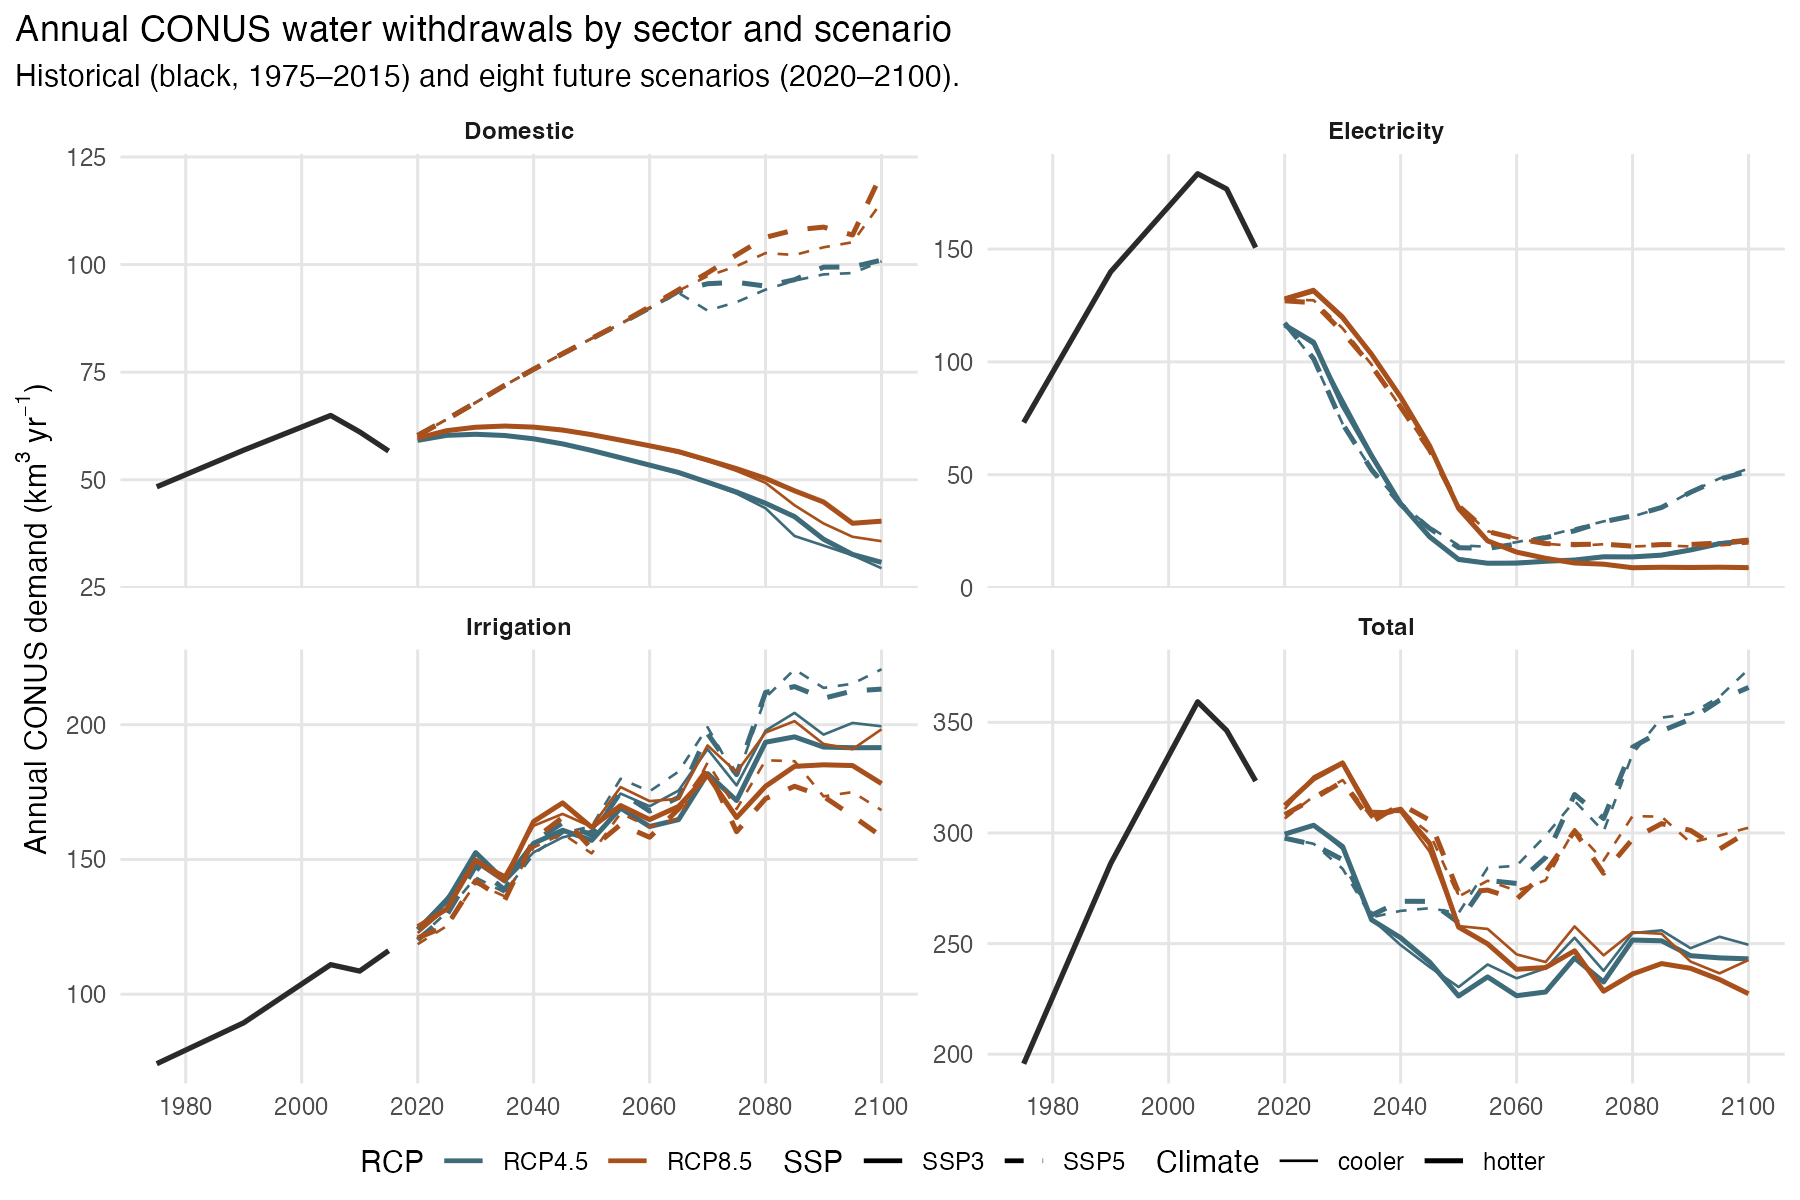
\includegraphics[width=\linewidth]{val6-scenarios-annual-conus-timeseries.png}
\caption{Annual CONUS water withdrawals by sector and scenario. \DIFdelbeginFL \DIFdelFL{Historical }\DIFdelendFL \DIFaddbeginFL \DIFaddFL{The historical }\DIFaddendFL simulation (black, \DIFdelbeginFL \DIFdelFL{1975--2015}\DIFdelendFL \DIFaddbeginFL \DIFaddFL{1975--2019}\DIFaddendFL ) is \DIFdelbeginFL \DIFdelFL{shown alongside }\DIFdelendFL \DIFaddbeginFL \DIFaddFL{connected to each of the }\DIFaddendFL eight future scenarios (2020--2100) \DIFdelbeginFL \DIFdelFL{that }\DIFdelendFL \DIFaddbeginFL \DIFaddFL{at 2019 so the hand-off is continuous in the visual; future scenarios }\DIFaddendFL vary by RCP (color), climate-model sample (line width), and SSP (line style). Each panel uses an independent $y$-axis.}
\label{fig:scenarios}
\end{figure}

\DIFaddbegin \subsection*{\DIFadd{HDD/CDD threshold sensitivity (Eq.~\ref{eq:elec-cases})}}

\DIFadd{The piecewise definition in Eq.~(\ref{eq:elec-cases}) classifies each cell-year into one of four cases by comparing annual HDD and CDD totals against the thresholds $H_{\mathrm{thr}}=650$ and $C_{\mathrm{thr}}=450$ from Huang et al.}\cite{Huang2018}\DIFadd{. We tested the sensitivity of the case partition and the resulting CONUS-aggregate monthly Electricity weight profile to perturbing the thresholds by $\pm 50\%$, holding the GCAM-USA shares $(p_{\mathrm{heat}}, p_{\mathrm{cool}}, p_{\mathrm{other}})$ fixed at $(0.20, 0.40, 0.40)$. Under the default thresholds, 32\% of CONUS cell-years fall in case~1 (both heating and cooling seasons present), 46\% in case~2 (heating only), 19\% in case~3 (cooling only), and 3\% in case~4 (uniform). Halving the thresholds to $(325, 225)$ moves the partition toward case~1 (49\%, 35\%, 16\%, 0\%); raising them by 50\% to $(975, 675)$ moves it toward case~2 (20\%, 54\%, 22\%, 5\%). The CONUS-aggregate monthly Electricity weight profile shifts by at most $\approx 1.8$ percentage points per month under either perturbation, with the largest changes concentrated in summer months (the low-threshold scenario raises the July weight by $\approx 1.8$~pp; the high-threshold scenario lowers it by $\approx 1.1$~pp). The case-4 cell-year fraction stays under 5\% in all three scenarios, so the uniform-fallback assumption is invoked rarely and is not a load-bearing source of uncertainty. Implementation and full diagnostics: }\texttt{\DIFadd{tethys\_integration\_metarepo/sensitivity/eq5-hdd-cdd-thresholds.py}}\DIFadd{; outputs at }\texttt{\DIFadd{figures/eq5-hdd-cdd-sensitivity-summary.csv}}\DIFadd{, }\texttt{\DIFadd{figures/eq5-hdd-cdd-sensitivity-monthly-profile.csv}}\DIFadd{, and Figure~\ref{fig:eq5-sensitivity}.
}

\begin{figure}[ht]
\centering
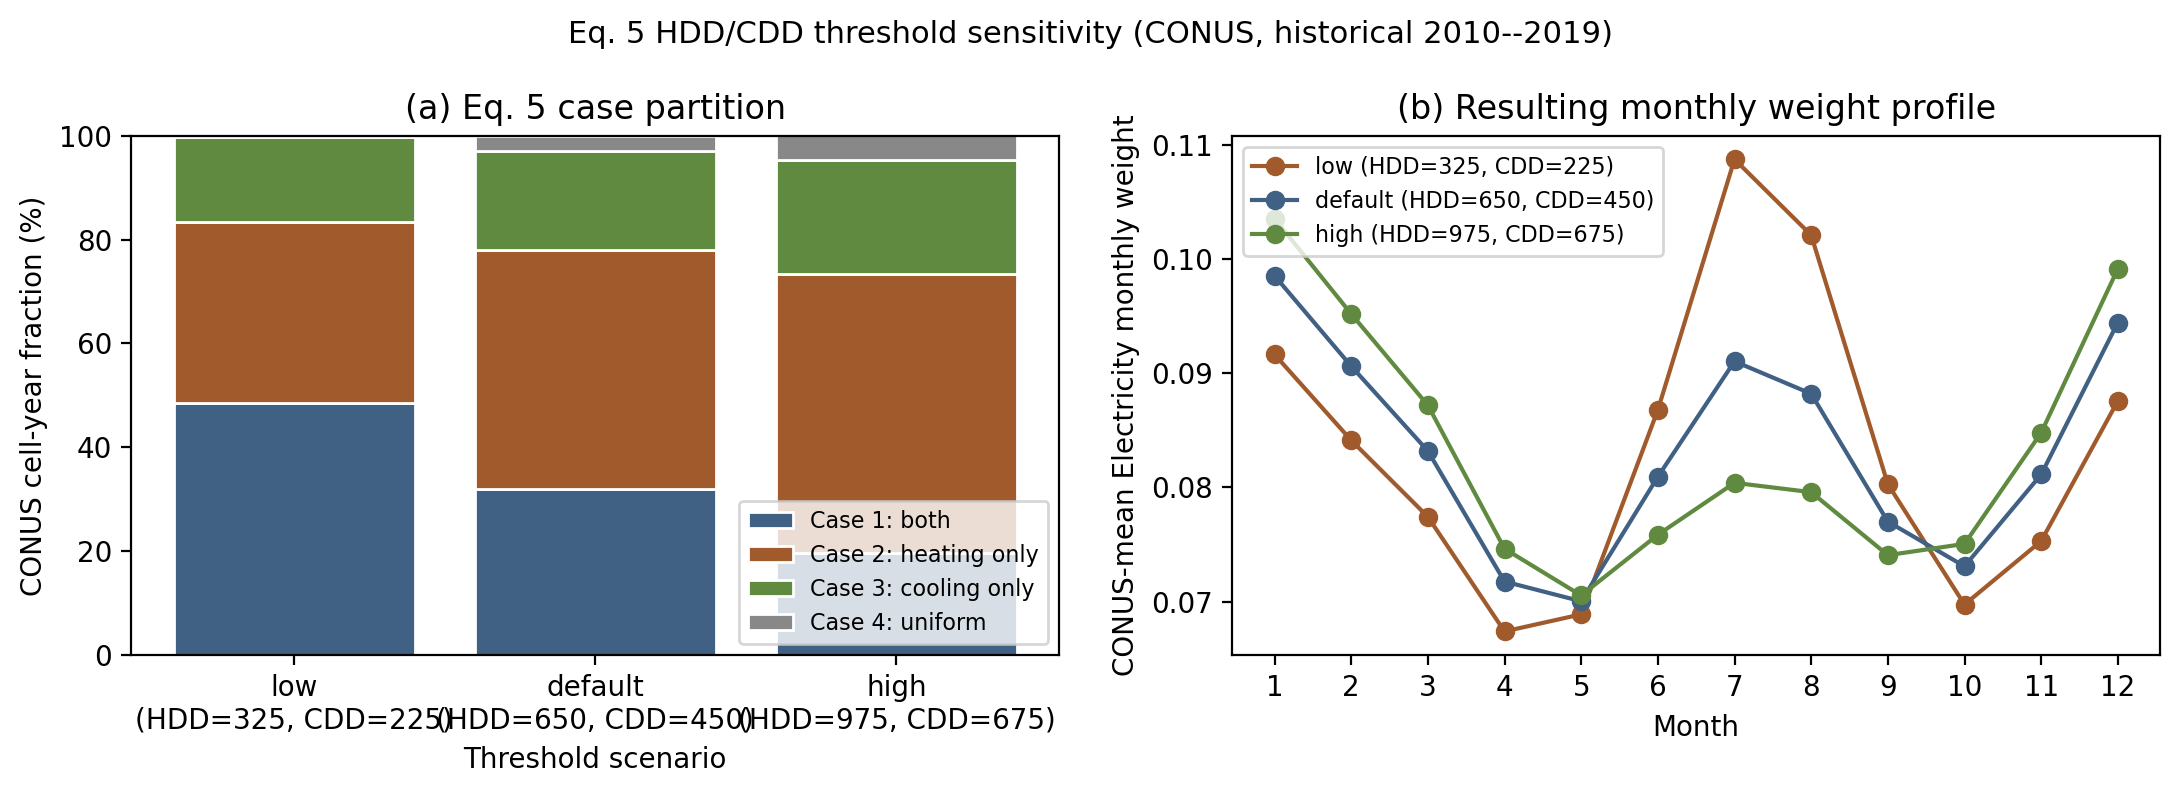
\includegraphics[width=\linewidth]{eq5-hdd-cdd-sensitivity.png}
\caption{\DIFaddFL{Sensitivity of Eq.~(\ref{eq:elec-cases}) to the HDD/CDD thresholds, computed over CONUS for the historical reference decade (2010--2019). (a) Stacked partition fractions of cell-years into the four cases under the default $(650, 450)$ thresholds and $\pm 50\%$ perturbations. (b) CONUS-mean Electricity monthly weight profile resulting from each threshold pair, holding the GCAM-USA $(p_{\mathrm{heat}}, p_{\mathrm{cool}}, p_{\mathrm{other}})$ shares fixed at $(0.20, 0.40, 0.40)$ to isolate the sensitivity to the case partition.}}
\label{fig:eq5-sensitivity}
\end{figure}

\DIFaddend \subsection*{Limitations}

Several known limitations should inform reuse of the dataset, grouped here into spatial-stationarity caveats and methodological caveats. \emph{Livestock spatial stationarity:} the GLW~3 livestock distribution is held fixed at 2010 across all years and scenarios. Livestock is \textasciitilde2\% of CONUS demand, but within individual basins --- particularly in states with rapidly shifting livestock composition --- this may introduce local bias. \emph{Manufacturing and mining proxy:} using population as the proxy for these two sectors captures average patterns of labor-associated demand but misses site-specific industrial or mining facilities whose water withdrawals can dominate local basin totals.

On the methodological side, the \emph{electricity source-share carve-out} in Eq.~(\ref{eq:source-shares}) assigns thermoelectric demand to surface water only and renormalizes remaining-sector shares; where a thermoelectric plant is served from a local groundwater source (rare but documented), this assumption places the withdrawal on surface water and slightly overstates surface demand elsewhere. \emph{Riparian vs.\ reservoir allocation:} the dataset represents demand at the cell where use occurs, which is not necessarily the cell from which water is withdrawn in reservoir-fed or interbasin-transfer systems; downstream routing and water-management models (e.g., mosartwmpy) handle the supply-side re-allocation. The \emph{simplified GSI} used for irrigation temporal downscaling (Eqs.~\ref{eq:gsi-components}--\ref{eq:gsi-monthly}) drops the vapour-pressure-deficit (VPD) component of the original Jolly et al.\cite{Jolly_2005} formulation; this simplification is consistent with Moore et al.\cite{Moore_2015} but may underweight drought months in humid climates where VPD is the binding constraint. \emph{Conveyance losses:} irrigation files exist with and without conveyance losses applied (\texttt{\_with\_losses} suffix), and users coupling the dataset to hydrologic routing should select the appropriate variant for their application. \emph{GCAM-USA temporal interpolation:} the 5-year GCAM step linearly interpolated to annual resolution suppresses interannual variability and is most visible as smoother trend lines in irrigation, which makes the dataset appropriate for scenario-level and climatological-mean analyses but not for replicating year-to-year demand variability.

% -----------------------------------------------------------------------------
\section*{Usage Notes}

We distribute the dataset as netCDF~4 files. A typical Python workflow loads one scenario file and computes a CONUS total:
\begin{verbatim}
import xarray as xr
ds = xr.open_dataset(
    "rcp45cooler_ssp3/Domestic_withdrawals_monthly.nc"
)
# CONUS total by year and month:
total = ds["Domestic"].sum(dim=("lat", "lon"))
\end{verbatim}
The result is a (year, month) array of CONUS-total Domestic withdrawals in km$^3$~yr$^{-1}$. Users convert from the native unit (km$^3$~yr$^{-1}$) to MGD by multiplying by $264{,}172.05124/365$, so $1\text{ km}^3\text{ yr}^{-1} \approx 723.76$~MGD.

The companion integration meta-repository provides HUC-level aggregation in \texttt{validation/1-postprocess-tethys.py}, which uses the \texttt{xagg} library to compute overlap-weighted aggregates from the 1/8$^{\circ}$ grid to HUC2, HUC4, HUC6, HUC8, or HUC12 polygons.

The dominant water-use sector at each \DIFdelbegin \DIFdel{cell (}\DIFdelend \DIFaddbegin \DIFadd{1/8$^{\circ}$ cell shown in }\DIFaddend Figure~\ref{fig:dominant-sector} \DIFdelbegin \DIFdel{) summarizes how this dataset's }\DIFdelend \DIFaddbegin \DIFadd{(front of paper) is one example product that exercises the full }\DIFaddend multi-sector resolution\DIFdelbegin \DIFdel{at 1/8$^{\circ}$ --- with explicit groundwater/surface-water shares --- differs from }\DIFdelend \DIFaddbegin \DIFadd{; }\DIFaddend the prior Tethys global product \DIFdelbegin \DIFdel{, whose advances we itemize }\DIFdelend \DIFaddbegin \DIFadd{cannot reproduce this multi-sector mosaic at this resolution, and the advances that make it possible are itemized }\DIFaddend next.

\DIFdelbegin %DIFDELCMD < \begin{figure}[ht]
%DIFDELCMD < \centering
%DIFDELCMD < 
\includegraphics[width=\linewidth]{usage1-dominant-sector-tethys-grid.png}
%DIFDELCMD < %%%
%DIFDELCMD < \caption{%
{%DIFAUXCMD
\DIFdelFL{Dominant water-use sector at each 1/8$^{\circ}$ cell, by annual-average consumption.}}
%DIFAUXCMD
%DIFDELCMD < \label{fig:dominant-sector}
%DIFDELCMD < \end{figure}
%DIFDELCMD < 

%DIFDELCMD < %%%
\DIFdelend \section*{Improvements over previous version}

Compared with the prior Tethys global product\cite{Khan2023}, the dataset presented here advances the representation of demand in six specific ways.

\paragraph{GCAM-USA integration.} The prior record used the global GCAM configuration, which disaggregated U.S.~demand from a single national total. This dataset uses GCAM-USA, which resolves U.S.~electricity generation, manufacturing, and municipal demand at the state level and crop irrigation demand at state$\,\times\,$basin intersections. State-level inputs eliminate the artifact of national-average demand being pushed uniformly into states with very different sectoral mixes, and they allow the subsequent spatial downscaling to respect state-level regulatory and policy boundaries.

\paragraph{CERF-based power-plant siting.} Prior gridded electricity demand used population as the spatial proxy, which approximates the location of load rather than the location of cooling demand. This dataset uses explicit power-plant siting from the CERF model\cite{Vernon2021}, which places thermoelectric plants at $\approx$1-km resolution based on siting feasibility (exclusion layers, transmission proximity, cooling-water access) and then aggregates installed capacity to the 1/8$^{\circ}$ grid as the proxy. The result places thermoelectric demand at actual generation sites rather than at population centroids, correcting the historical decoupling of load from generation in regions like the lower Colorado and Tennessee Valley.

\paragraph{SSP-consistent population.} Prior work used a static base-year population map to distribute municipal, manufacturing, and mining demand across all years, including future projections. This dataset uses SSP3 and SSP5 gridded population projections from Jones and O'Neill\cite{Jones_2016}, linearly interpolated from their decadal native resolution to annual values. Scenario-consistent population is essential for the SSP-differentiated futures: SSP3 and SSP5 diverge markedly in U.S.~population growth, and that divergence propagates into the public-supply demand field in a way that a static map cannot represent.

\paragraph{GSI-based irrigation temporal downscaling.} Prior irrigation monthly weights used a simpler temperature-driven scheme. This dataset computes per-cell monthly weights (Eq.~\ref{eq:irr-weights}) from the TGW-WRF monthly deficit and growing-season index, so the monthly distribution of irrigation demand responds to climate-consistent drought and growing-condition signals rather than to a static seasonal template. The monthly irrigation distribution thus varies from year to year and across scenarios, tracking interannual drought variability that a static template cannot reproduce.

\paragraph{USGS-anchored source-share attribution.} Prior work applied GCAM's basin-level renewable vs.\ non-renewable split uniformly across cells within each basin. This dataset uses Eq.~(\ref{eq:source-shares}) to anchor the historical 2015 spatial pattern to USGS baseline observations while preserving the temporal evolution from GCAM. In regions with observable baseline data this reduces bias relative to the GCAM-uniform allocation (see Technical Validation); outside those regions, the GCAM share is preserved.

\paragraph{Resolution refinement.} Spatial resolution is refined from 1/2$^{\circ}$ to 1/8$^{\circ}$, a factor-of-4 improvement per dimension and a factor-of-16 improvement in areal resolution. Combined with the finer proxy data (CERF plants at \textasciitilde1~km, Demeter LULC at 1/8$^{\circ}$, Jones population at 1/8$^{\circ}$), the 1/8$^{\circ}$ grid allows the resulting demand field to represent sub-state variation relevant to river routing, reservoir management, and local planning applications.

Together, these six advances produce a dataset that captures HUC6 spatial pattern (annual correlations of \DIFdelbegin \DIFdel{0.71}\DIFdelend \DIFaddbegin \DIFadd{0.73}\DIFaddend --0.95) and supports detailed scenario analysis against the refreshed January~2025 USGS water-use record, which includes updated thermoelectric cooling-water estimates\cite{skinnerWaterWithdrawalConsumption2025}. As discussed in Technical Validation, the close \DIFdelbegin \DIFdel{CONUS-aggregate agreement masks compensating sector-level biases --- a $-45\%$ underestimate in Domestic and a $-30\%$ underestimate in Electricity withdrawals partially offset by a $+5\%$ bias in Irrigation --- so }\DIFdelend \DIFaddbegin \DIFadd{per-sector mean-bias agreement (within $\pm 7\%$) masks substantial within-basin spread (NRMSE 68--171\%, MedAPE 37--86\%); }\DIFaddend downstream users computing per-sector scarcity \DIFaddbegin \DIFadd{at individual basins }\DIFaddend should consult Table~\ref{tab:validation-metrics} \DIFaddbegin \DIFadd{and the HUC6 maps }\DIFaddend rather than rely on aggregate agreement alone.

% -----------------------------------------------------------------------------
\section*{Code and external data availability}

We release all code under open-source licenses (BSD-2 for Tethys; permissive licenses for the other components, see each repository).
\begin{itemize}
    \item \textbf{Tethys downscaling package}: \url{https://github.com/JGCRI/tethys} (\texttt{pip install tethys-downscale}). Each scenario YAML config records the exact \texttt{tethys-downscale} version used to produce that scenario's outputs.
    \item \textbf{Integration meta-repository}: \url{https://github.com/IMMM-SFA/tethys_integration_metarepo}. Contains the per-scenario run drivers (\texttt{scripts/1\_runs/im3\_tethys\_runs/}), climate-forcing preprocessing (\texttt{scripts/0\_preprocessing/gsi\_nersc/} and \texttt{scripts/0\_preprocessing/compute\_\{gsi,deficit,monthly\_weights\}.py}), runoff-share adjustment (\texttt{scripts/2\_postprocess/adjust\_runoff\_shares/}), and the numbered validation pipeline (\texttt{validation/}).
    \item \textbf{Demeter} (land-use downscaling, used to produce per-crop irrigated-area proxies): \url{https://github.com/IMMM-SFA/demeter}\cite{Vernon-2018}.
    \item \textbf{CERF} (power-plant siting): \url{https://github.com/IMMM-SFA/cerf}\cite{Vernon2021}.
\end{itemize}
The TGW-WRF climate forcing\cite{Jones2023TGW} that drives the Tethys runs is available as external data at \url{https://tgw-data.msdlive.org/}. To reproduce the published record for one scenario, see the README of the integration meta-repository, which documents required inputs, expected outputs, and the command sequence for each stage.

% -----------------------------------------------------------------------------
\section*{Acknowledgments}

This research was supported by the U.S.~Department of Energy, Office of Science, as part of research in MultiSector Dynamics, Earth and Environmental System Modeling Program. We thank the TGW-WRF team for the downscaled climate product, the GCAM-USA team for the scenario simulations, and the USGS water-use program for the reference observations used in validation.

\section*{Author contributions statement}

% TODO: coauthors to fill in per CRediT roles. Illustrative template:
C.B.~Coordinated the downscaling runs, conducted the HUC-scale validation, and drafted this version of the manuscript based on an earlier draft by I.T.
H.N.~Developed and maintained the Tethys model, conducted the runs, and helped with the interpretation of GCAM-USA and Tethys outputs.
T.T.~Extended the Tethys package to support GCAM-USA inputs, developed the first version of the Tethys metarepo, and carried out the initial scenario runs.
I.T.~Wrote initial draft of this manuscript, contributed to the CERF--Tethys integration and power-plant proxy construction.
K.T.~Developed the USGS-anchored source-share attribution as a postprocessing to Tethys and conducted runs.
H.E.~Produced the TGW-WRF preprocessing pipeline for PET, HDD/CDD, and GSI.
K.M.~Developed CERF--Tethys integration and power-plant proxy construction.
N.V.~Contributed to scenario design and interpretation.
N.S.~Project management, scenario design and interpretation.
J.R.~Provided overall project guidance and scientific review.

\section*{Competing interests}

The authors declare no competing interests.

\bibliography{Tethys}

\end{document}
